\documentclass[t]{beamer}

\mode<presentation>{
\usetheme[numbers,totalnumber,compress,sidebarshades]{PaloAlto}
\setbeamercovered{transparent}
\definecolor{kuviolet}{RGB}{172, 19, 108	}
\definecolor{kuvioletlys}{RGB}{238, 130, 238}
\definecolor{kuvioletlyslys}{RGB}{173,190,177}
\definecolor{kuvioletlyslyslys}{RGB}{214,223,216}
\logo{
\includegraphics[width=1.5cm]{unicaen1.png}}
}

\setbeamertemplate{footline}[frame number]

  \usecolortheme[named=kuviolet]{structure}
  \useinnertheme{circles}
  \usefonttheme[onlymath]{serif}
  \setbeamercovered{transparent}
  \setbeamertemplate{blocks}[rounded][shadow=true]

\usepackage{pslatex}

\usepackage[utf8]{inputenc}
\usepackage[T1]{fontenc}
\usepackage[frenchb]{babel}
 \usepackage{xcolor}
  \usepackage{color}
\usepackage{gensymb}

\title{Robot Ricochet Solver}
\author[]{SI-MOHAMMED Sonia-Taous \\ BOUAOUD Malik \\ AIT KHEDDACHE Wissam \\ SINI Lynda \\ CUQUEMELLE Mathieu \\[\baselineskip] \small{{\color{kuviolet} Encadré par :}
  \and \\ M.BONNET Gregory \\ M.CHATEL Romain \\ M.SASSI Taoufik }}
  
\setbeamertemplate{footline}[frame number]%pour changer le pied de page par un affichage des numéros de slide

\setbeamertemplate{frametitlecontinuation}{\insertcontinuationcountroman}
\setbeamertemplate{frametitlecontinuation} {\insertcontinuationcount} 

\setbeamertemplate{navigation symbols}{%
\insertslidenavigationsymbol
\insertframenavigationsymbol
\insertsubsectionnavigationsymbol
\insertsectionnavigationsymbol
\insertdocnavigationsymbol
\insertbackfindforwardnavigationsymbol
}

\AtBeginSection[]{
  \begin{frame}{Sommaire}
  \small \tableofcontents[currentsection, hideothersubsections]
  \end{frame} 
}

\begin{document}
\begin{frame}
\frametitle{Conception logicielle avancée}
\framesubtitle{L2 informatique 2019/2020}
\titlepage
\end{frame}
%\maketitle

%--------------------
\begin{frame} 
\frametitle{Plan}
\tableofcontents
\end{frame}
%----------------------------------------------------------------------Introduction---------------------------------------------------------------------------------

\section{Introduction}
\subsection{Robot Ricochet Solver, c'est quoi?}
\begin{frame}
\frametitle{Description du jeu}
\framesubtitle{Écran Principal}
\begin{center}
\begin{figure}[h!]
\centerline{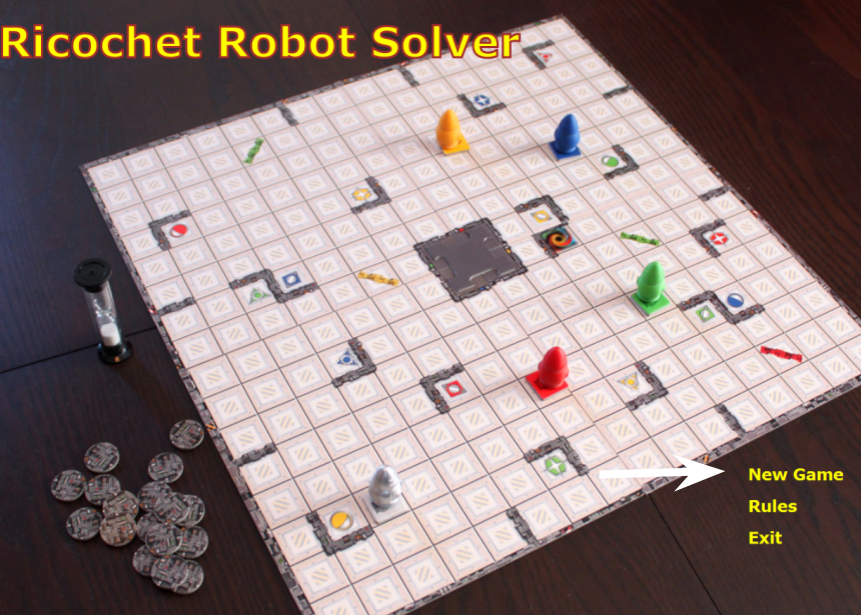
\includegraphics[scale=0.35]{ecranPrincipal.png}}
\caption{L'écran principal du jeu.}
\end{figure}
\end{center}
\end{frame}

\begin{frame}
\frametitle{Description du jeu}
\framesubtitle{Règles du jeu}
\begin{center}
\begin{figure}[h!]
\centerline{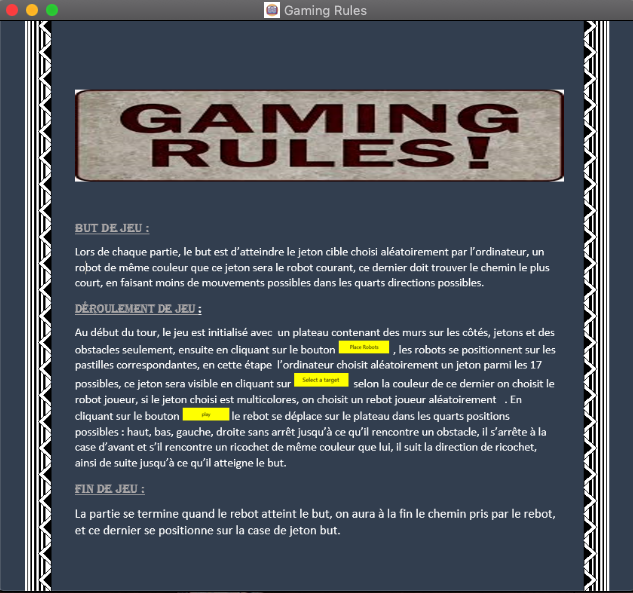
\includegraphics[scale=0.28]{rules.png}}
\caption{Le clic sur le bouton \textbf{Rules}, provoque l'affichage de la fenêtre où on explique les règles du jeu.}
\end{figure}
\end{center}
\end{frame}

\begin{frame}
\frametitle{Description du jeu}
\framesubtitle{Plateau}
\begin{center}
\begin{figure}[h!]
\centerline{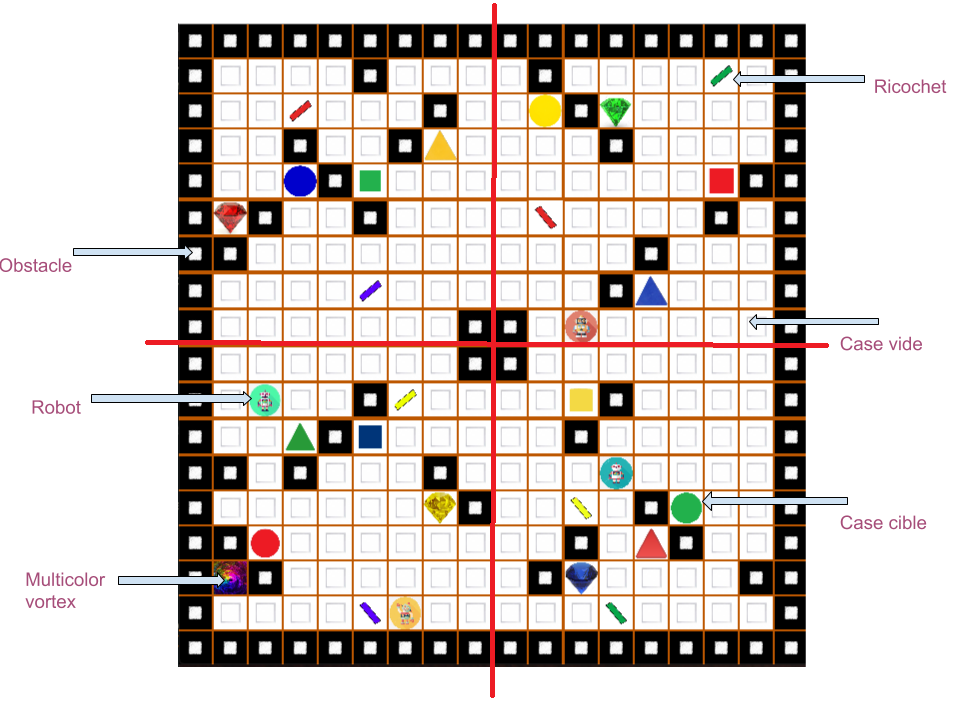
\includegraphics[scale=0.45]{gridDesc.png}}
\caption{Le clic sur le bouton \textbf{NewGame} provoque la création et l'affichage du plateau du jeu.}
\end{figure}
\end{center}
\end{frame}



\begin{frame}
\frametitle{Description du jeu}
\framesubtitle{Chargement du plateau de jeu}
\begin{figure}
\begin{columns}[t]
\column{.3\textwidth}
\centering
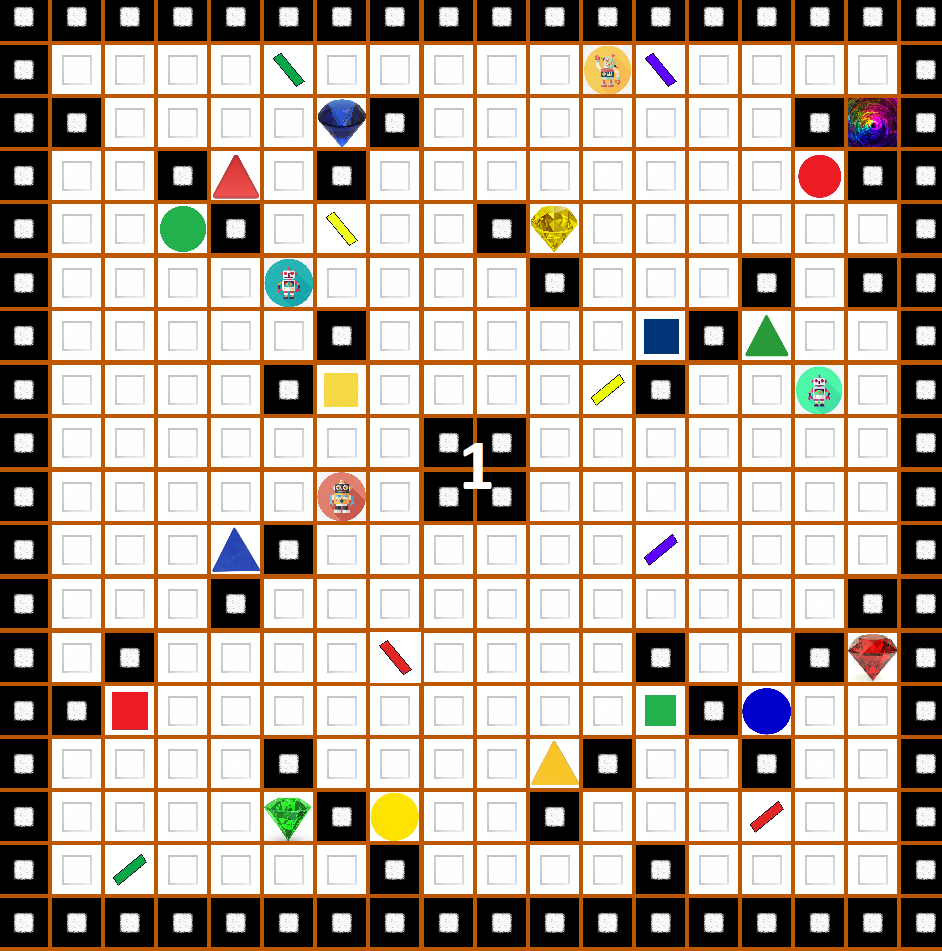
\includegraphics[width=4cm,height=4cm]{plat1.png}
\column{.4\textwidth}
\centering
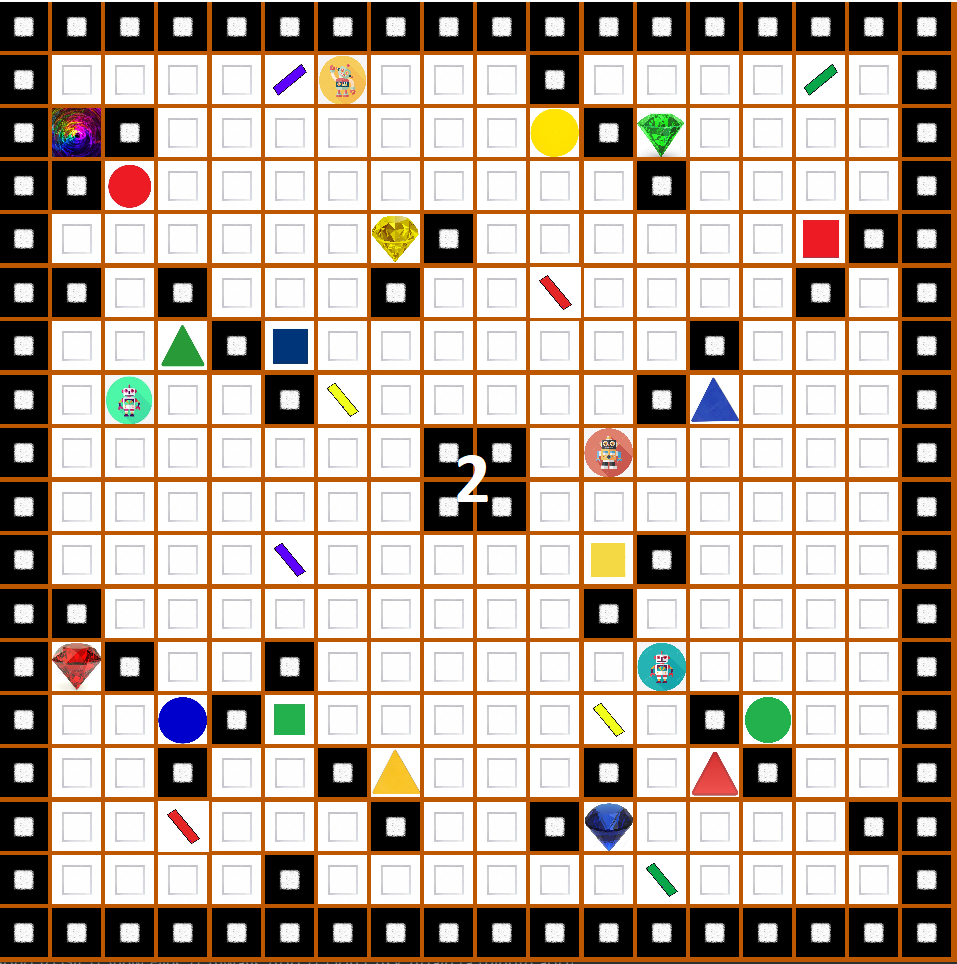
\includegraphics[width=4cm,height=4cm]{plat2.png}
\end{columns}
\caption{Exemple de deux plateaux possibles.}
\end{figure}
\begin{alertblock}{Remarque}
Nous avons un total de 24 plateaux de jeu possible.
\end{alertblock}
\end{frame}

\begin{frame}
\frametitle{Description du jeu}
\framesubtitle{Chargement du plateau de jeu }
\begin{block}{Création du plateau de jeu }
Comme vous pouvez le constater ci-dessus, à chaque début de partie le plateau change, cela est du au choix aléatoire des 4 sous-plateaux ,formant le plateau final du jeu.
\end{block}
\begin{alertblock}{Remarque}
Une rotation des sous-plateaux implique dans deux cas une inversion des ricochets. Ces deux cas représentent la rotation du sous-plateau haut-droit et bas-gauche.
En effet, une rotation de 90\degree, implique le changement de direction de tous les ricochets. En revanche une rotation de 180\degree, ne change rien à ces derniers.
\end{alertblock}
\end{frame}




\begin{frame}
\frametitle{Description du jeu}
\framesubtitle{But et règles du jeu}
\begin{block}{But du jeu}  
\begin{itemize}
\item Déplacer un robot jusqu’à la case cible choisie, avec un minimum nombre de déplacements.
\end{itemize}
\end{block}
\begin{block}{Règles du jeu}  
 \begin{itemize}
\item Les sous-plateaux sont choisis aléatoirement à chaque début de partie.
\item Le robot peut se déplacer horizontalement ou verticalement.
\item Le robot et la case cible sont de même couleur.
\item Les obstacles sont : une case obstacle, ou un autre robot.
\item Les ricochets changent la direction du robot.
\item Un jeton est choisi aléatoirement.
\end{itemize}
\end{block}
\end{frame}



\begin{frame}
\frametitle{Description du jeu}
\framesubtitle{Exemple}
\begin{exampleblock}{Exemple } 
Prenons l'exemple du chemin, que le robot vert doit emprunter, pour arriver jusqu'au triangle vert !
\end{exampleblock}
\begin{center}
\begin{figure}[h!]
\centerline{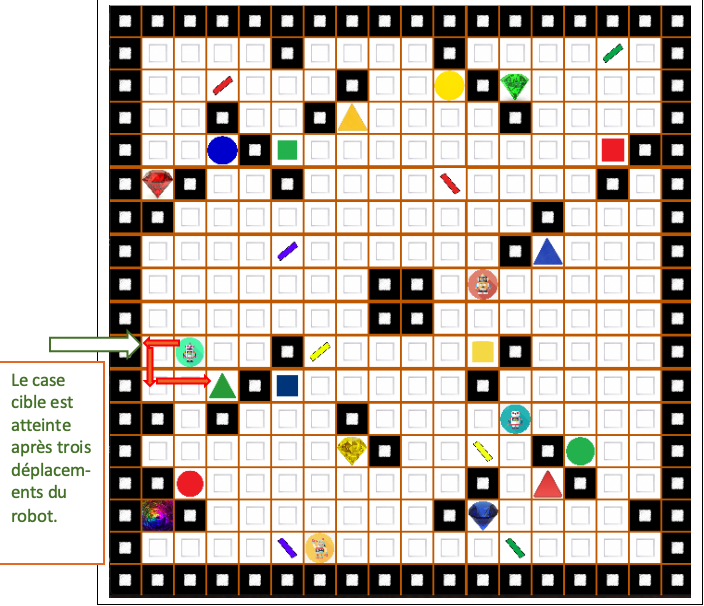
\includegraphics[scale=0.24]{cheminEx.png}}
\end{figure}
\end{center}
\end{frame}
\subsection{Problème}
\begin{frame}
\frametitle{Problème}
\begin{center} 
Comment peut-on déplacer le robot jusqu'au but, avec un minimum de coups possibles?
\end{center}
\end{frame}


%---------------------------------------------------Elements techniques-----------------------------------------------------------------------------------------

\section{Éléments techniques}
\subsection{Algorithme A*}
\begin{frame}
\frametitle{Algorithme A*}
\framesubtitle{Heuristique}
\begin{block}{Définition}
C'est un calcul de la distance qui sépare chaque nœud du but , ceci est pour estimer le meilleur chemin .
\end{block}
\begin{block}{Heuristique utilisée }
Dans notre implémentation, on a utilisé la distance de Manhattan comme heuristique. 
\begin{equation}H(n) = abs(x) + abs(y)\end{equation}
\end{block}
\end{frame}

\begin{frame}
\frametitle{Algorithme A*}
\framesubtitle{Principe}
\begin{block}{Présentation}
L'algorithme A* sert a rechercher un chemin dans un graphe entre deux nœuds : initial et final, en évaluant l'heuristique sur chaque nœud afin de trouver le meilleur chemin.
\end{block}
\begin{exampleblock}{Exemple } 
Appliquant A* sur l'exemple donné ci-dessous, en calculant l'heuristique pour chaque nœud.
\end{exampleblock}
\end{frame}

\begin{frame}
\frametitle{Algorithme A*}
\framesubtitle{Principe}
\begin{center}
\begin{figure}[h!]
\centerline{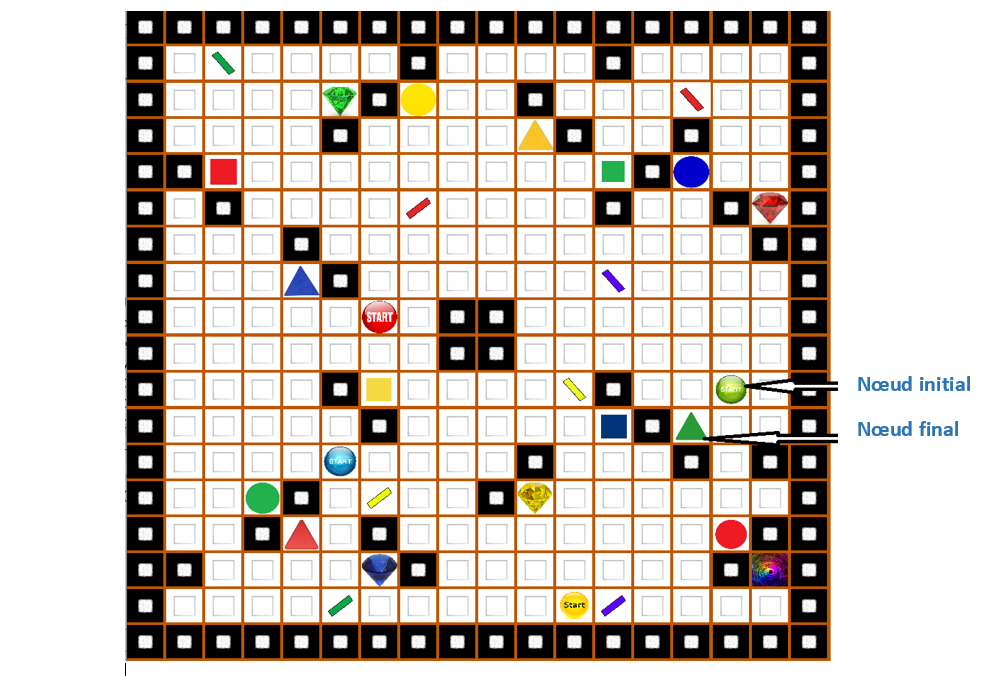
\includegraphics[scale=0.4]{Avant.PNG}}
\caption {L'exemple étudié ci-dessous}
\end{figure}
\end{center}
\end{frame}

\begin{frame}
\frametitle{Algorithme A*}
\framesubtitle{Principe}
\begin{center}
\begin{figure}[h!]
\centerline{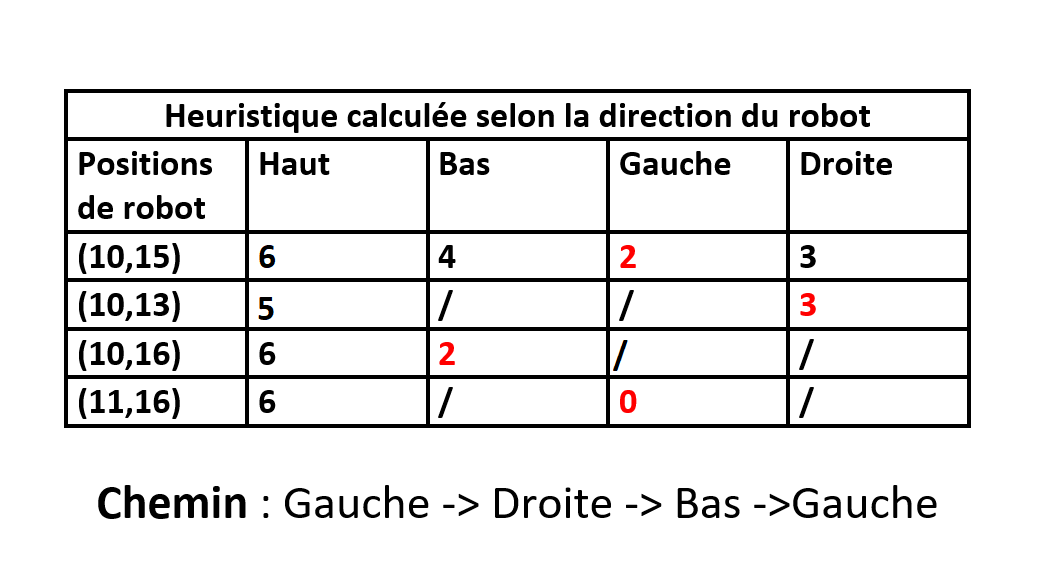
\includegraphics[scale=0.5]{heuristique.PNG}}
\end{figure}
\end{center}
\begin{center}
On choisit le nœud ayant la plus petite heuristique, les "/" représente les nœuds déjà visités, donc inutile de recalculer leur valeurs.
\end{center}
\end{frame}

\begin{frame}
\frametitle{Algorithme A*}
\framesubtitle{Heuristique}
\begin{figure}[h!]
\centerline{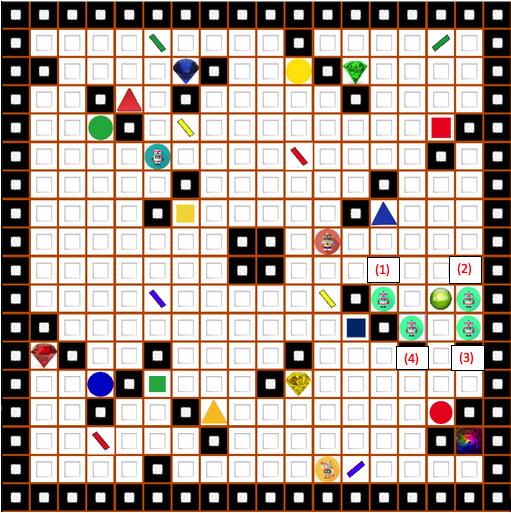
\includegraphics[scale=0.33]{apres.PNG}}
\caption{Le chemin obtenu après l'application de A*.}
\end{figure}
\end{frame}



\begin{frame}
\frametitle{Tables de transposition}
\framesubtitle{Description}
\begin{block}{Definition}
Une table de transposition est un graphe de positions avec leurs évaluations, ou un noeud déjà visité n'est pas étendu et réévalué.
\end{block}
\begin{exampleblock}{Utilité } 
Dans notre implémentation de l'algorithme A* ,nous utilisons 2 HashMaps gScore et fScore (current2 startCosts et cheapestCost) qui représentent notre table de transposition permettant de faire gagner en rapidité l'algorithme, puisque ce dernier ne s'appliquera pas sur des nœuds déjà évalués. Et met en priorité les nœuds non visités avec l'heuristique la plus basse, jusqu'à atteindre le but.
\end{exampleblock}
\end{frame}

\subsection{Tables de transposition}
\begin{frame}
\frametitle{Tables de transposition}
\framesubtitle{Déroulement}
\begin{center}
\begin{figure}[h!]
\centerline{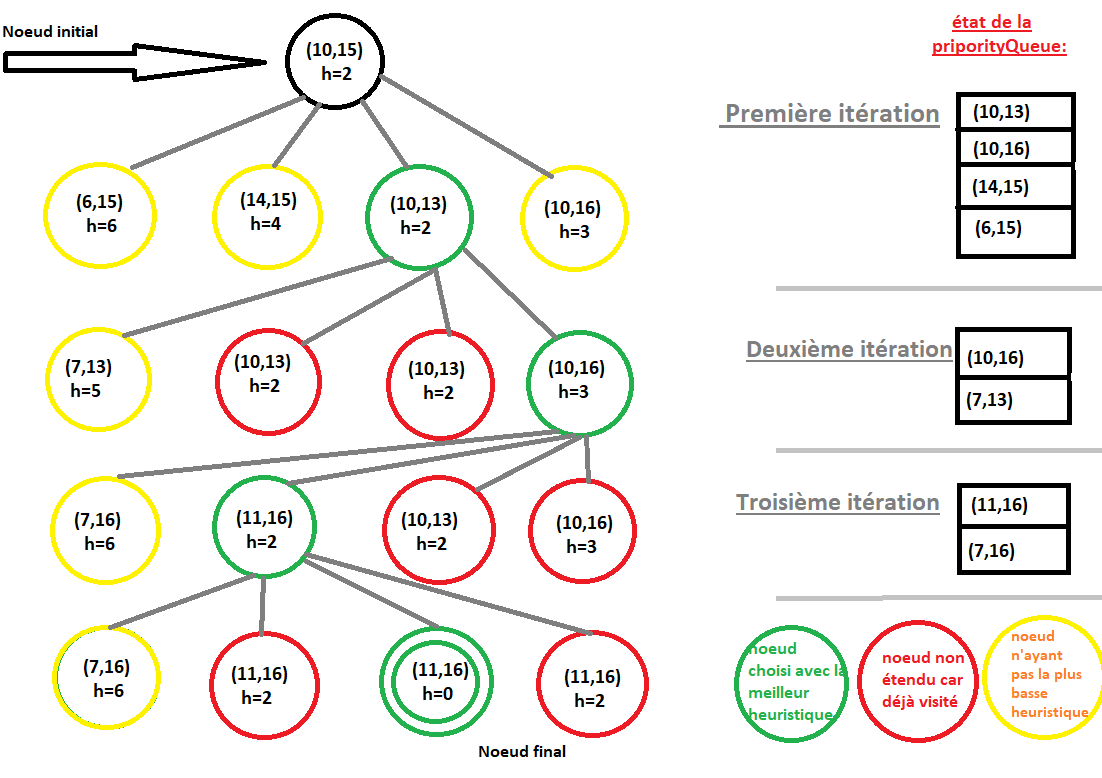
\includegraphics[scale=0.5]{tableDeTransposition.png}}
\end{figure}
\end{center}
\end{frame}

\begin{frame}
\frametitle{PriorityQueue}
\framesubtitle{Remarque}
\begin{center}
\begin{alertblock}{Remarque } 
Il est important de comprendre que si un nœud déjà visité ne sera pas ajouté à la PriorityQueue \textit{voir l'exemple ci-dessus}, et que chaque itération repose sur le retrait du premier élément de cette structure puisqu'il a l'heuristique la plus intéressante, et donc ce nœud sera évalué à la prochaine itération.
\end{alertblock}
\end{center}
\end{frame}

%--------------------
\section{Conclusion}
\begin{frame}
\frametitle{Conclusion}
\begin{center}
\begin{block}{Pour conclure } 
L’objectif du projet était de développer une application "Java" pour le jeu "Ricochet Robot Solver", tout en implémentant l'Algorithme de recherche de chemin A* en utilisant les tables de transposition, nous avons reussis à relever le defis,tout en ajoutant quelques bonus notamen le \textit{Design pattern Singleton} ou bien l'effet sonor.
\\Merci pour votre attention.
\end{block}
\end{center}
\end{frame}


\end{document}
